%\ifWithResults

\subsection{Results and Conclusion}

%%%%%%%%%%%%%%%%%%%%%%%%%%%%%%%%%%%%%%%%%%%%%%%%%%%%%%%%%%
\begin{frame}[t]{Results: Benchmarks}
 \small
    \begin{table}[ht]
    \centering
        \begin{tabular}{|c|c|c|}
        \hline
        \begin{tabular}[c]{@{}c@{}}Benchmark\\ name\end{tabular} & BM1, \% & BM2, \% \\ \hline
    within a socket                                          & 7.61    & 13.84   \\ \hline
    among sockets                                          & 9.04    & 26.26   \\ \hline
    among nodes                                            & -2.06   & 3.20    \\ \hline
    \end{tabular}
    \caption{Time reduction in comparison with the default approach}
        \label{table:benchmark:performance-gain}
    \end{table}

    \vspace{-20.0pt}
    \begin{figure}[htpb]
        \centering
        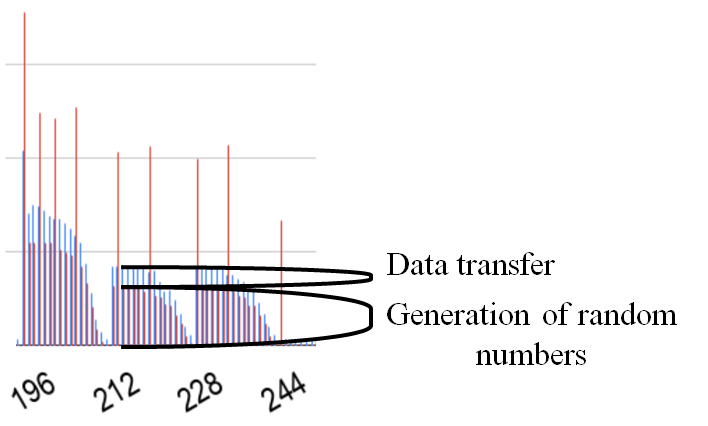
\includegraphics[width=0.6\textwidth]{figures/chapter-3/fast-data-transfer.png}
        \caption{\textbf{Intra-node} communication in case of \textbf{cube-64}}
    \end{figure}
\end{frame}

%%%%%%%%%%%%%%%%%%%%%%%%%%%%%%%%%%%%%%%%%%%%%%%%%%%%%%%%%%
\begin{frame}[t]{Results: ATHLET}
    \small
    \justifying
    
    \begin{itemize}
        \item Ideas, expressed in \textbf{BM2} benchmark,  were \textbf{implemented in ATHLET-NuT}
        
        \item Several simulation scenarios were taken for the final \textbf{verification and performance} testing
        
        \item \textbf{Verification} of the modified code \textbf{did not detect any deviations} of numerical results
        
        \item All tests showed  \textbf{considerable improvement} with respect to the \textit{\textbf{communication time}} i.e. approximately in \textbf{50-60\%}
    \end{itemize}

    \begin{table}[ht]
        \centering
        \begin{tabular}{|c|c|c|c|}
        \hline
Test case                                                    & \multicolumn{3}{c|}{pwr-3d}           \\ \hline
Type & intra-soket & intra-node & inter-node \\ \hline
Time reduction, \%                                           & 42.55\%     & 66.17\%    & 76.03\%    \\ \hline
        \end{tabular}
        \caption{ATHLET Results of \textbf{pwr-3d} test case}
    \end{table}

\end{frame}


%%%%%%%%%%%%%%%%%%%%%%%%%%%%%%%%%%%%%%%%%%%%%%%%%%%%%%%%%%
\begin{frame}[t]{Results: Overall Performance improvement}
    \spc
    \justifying
    
        \begin{itemize}
            \setlength\itemsep{0.25cm}
            \item \textbf{Overall improvement} of applied changes \textbf{achieved} only \textbf{0.14\% in average}, regardless of client-server allocation
            
            \item \textbf{Profiling} showed the \textbf{communication} part of the original implementation \textbf{took} around \textbf{0.24\%} of the \textbf{total} matrix evaluation-transfer \textbf{time}
            
            \item \textbf{Computation} part takes almost \textbf{99.8\%}
        \end{itemize}
    
    \begin{block}{According to BM2 benchmark:}
        \begin{itemize}
            \item Time spent on data transfer is approximately \textbf{one fifth of the total time}
            
            \item The benchmark \textbf{generates} only \textbf{random numbers}
        \end{itemize}
    \end{block}
    
\end{frame}


%%%%%%%%%%%%%%%%%%%%%%%%%%%%%%%%%%%%%%%%%%%%%%%%%%%%%%%%%%
\begin{frame}[t]{Conclusion}
    \small
    \justifying
    
    \begin{itemize}
            \item The \textbf{initial goal} of improvement ATHLET-NuT communication during the compressed Jacobian transfers \textbf{has been achieved}
            \item \textbf{Negligible} overall performance \textbf{gain}
            \begin{itemize}
                \item A \textbf{wrong Hypotheses} at the beginning
                \item Absence of \textbf{Initial Profiling}
            \end{itemize}
    \end{itemize}
    
        \begin{figure}[htpb]
        \centering
        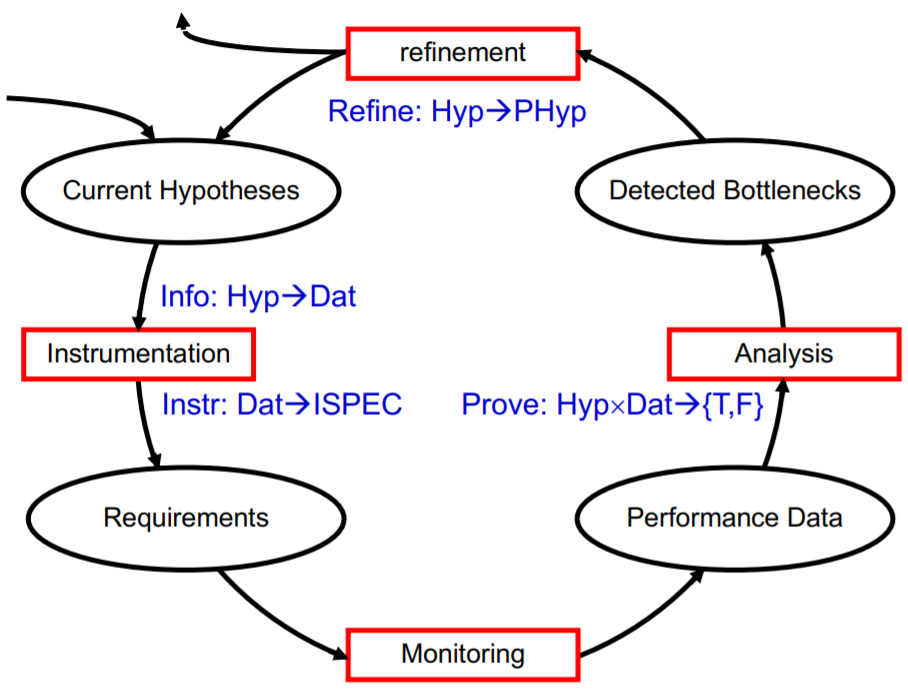
\includegraphics[width=0.44\textwidth]{figures/chapter-3/Performance-analysis.png}
        \caption{performance analysis framework \cite{perfomance-analysis-framework}}
    \end{figure}

\end{frame}
%\fi